% ----------------------------------------------------------
% Introdução (exemplo de capítulo sem numeração, mas presente no Sumário)
% ----------------------------------------------------------
% \chapter*{Introdução}
% \addcontentsline{toc}{chapter}{Introdução}
% ----------------------------------------------------------

\chapter{Introdução}\label{cap:introducao}

Citações podem ser feitas assim: \cite{Verdoold2014}

Ou então cite elas no meio da linha \citeonline{Agostinho2018}
sem parênteses.

Figuras podem ser referenciadas assim: Figura \ref{fig:a50p-5}

\begin{figure}[htb]
	\caption{\label{fig:a50p-5}Diagrama de Blocos do A50P-5.}
	\begin{center}
        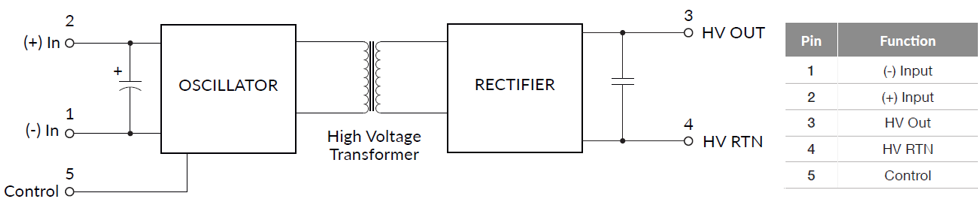
\includegraphics[width=\textwidth,trim=1 1 1 1,clip]{a50p-5.png}
	\end{center}
	\fonte{\cite{a50p-5}}
\end{figure}

\section{Objetivos} 

O objetivo 